\documentclass[12pt]{article}

\usepackage{setspace}
\usepackage{hyperref}
\usepackage{graphicx}
\usepackage{url}
\usepackage{xcolor}
\newcommand\todo[1]{\textcolor{red}{#1}}

\onehalfspacing

\parskip=2ex
\parindent=2em

\title{SWEN439 Visualisation Essay \\ John Snow's Cholera Map}
\author{Hai Tran 300224467}
\date{\today}

\begin{document}
\maketitle 

%Optional abstract
\begin{abstract}

During the nineteenth century, a disease called cholera had claimed many lives. There was no cure, and no one knew what was causing the disease. Doctors and scientists at the time believed that cholera was spread through miasma, however, a physician by the name of John Snow was not convinced. Snow believed that cholera was a waterborne disease spreading through contaminated water. In 1854, a cholera outbreak had broken out in London, causing over 600 fatalities. John Snow was convinced that cholera was a waterborne disease, yet could not convince anyone of it. Because of this, Snow investigated cases of cholera in his neighbourhood, plotting them on a map to test his hypothesis. Later, Snow's map would convince the world of the change that was needed, so much so, that Snow's map is said to be the birth of modern epidemiology. With Snow's famous map, it has influenced the way we visualise and map disease. Today, common techniques used to visual disease have been achieved through dot maps, choropleth maps, isopleth maps, and gradient maps.

\end{abstract}

\section{Introduction}
% This essay introduces John Snow's Cholera map, the history behind it, and the current state of research with respect to Snow's visualisation. 

This essay explores John Snow's cholera map visualising the 1854 cholera outbreak in London, England. The essay details the history of Snow's map and provides a description of the visualisation. In addition, it examines the influence that Snow's map has had on society, the questions it addresses, and the current state of research with respect to Snow's visualisation.

\section{The History of John Snow's Cholera Map}

In the nineteenth century, thousands of lives had been lost due to a disease called cholera. Although unknown at the time, cholera is caused by a bacteria called Vibrio cholerae, doubling in number every thirteen minutes and attacking the stomach and intestines \cite{channel1}. Symptoms include severe vomiting and diarrhea in victims, eventually causing an agonizing death to victims within hours \cite{heros, channel1}. During the time of the nineteenth century, there was no cure for cholera and no one knew what caused the disease. Doctors were convinced cholera was contracted through miasma: harmful airborne odours emanating from decaying waste, repulsive sewage or ``foul-smelling sites of organic decay" \cite{ucla, test}. This theory was based on observations that showed poorer areas being more susceptible to cholera, deaths in these regions more frequent \cite{heros}. A physician by the name of John Snow had an opposing view. Snow disbelieved the idea of cholera being spread by miasma, instead, hypothesising that cholera was a waterborne disease. In particular, Snow believed that cholera was spread by water contaminated from sewage \cite{ucla}. Snow came to this hypothesis after previously studying various outbreaks of cholera, writing academic papers that discussed his findings, yet no one believed him \cite{original}. Scientists and doctors gave little attention to Snow's work and were not convinced in Snow's theory, despite his findings \cite{ucla}. 

During the nineteenth century, 2.5 million people were estimated to be living in London. It was the largest city that had been built and contained the largest population at the time \cite{channel1, tedtalk}. An estimated third of the population lived in slums, up to 8 people in a room, and up to 40 to a house. Due to such a large population, this provoked filthy and unsanitary living conditions. People had cesspools containing fecal matter in their basements, eventually accumulating overtime. All this supported the idea that cholera was spread by miasma in the atmosphere due to the unsanitary living conditions. In an attempt to mitigate the smell, authorities created a law that made citizens empty their cesspools, expecting this to prevent cases of cholera \cite{tedtalk, johnson}. 

On the 28th of August, 1854, a cholera epidemic had broken out in the Soho district of London, England \cite{tedtalk}. After 3 days, 127 were found dead in London due to the epidemic. Within a few weeks, around 600 were estimated dead \cite{youtube, tedtalk}. Snow lived in the Soho district near the cholera outbreak and wanted to investigate his hypothesis of cholera being a waterborne disease. He suspected that if his hypothesis were true, incidents of the disease would involve a single source that everyone was going to, incidents of cholera clustering around the source of contamination such as a specific water pump \cite{test, tedtalk, johnson}. 

Snow tested his hypothesis by interviewing locals about cases relating to cholera with the help of Reverend Henry Whitehead. Through Reverend Whitehead, a socially connected individual, Snow was able to track down most cases of cholera \cite{tedtalk}. Snow searched for patterns, analysing data collected from the interviews, asking locals whether they knew victims had drunk from a specific water source, or whether they had not. He increasingly found people who drank from the Broad Street water pump were getting sick as opposed to everyone else. He also found that a brewery located near this pump had an independent water source where workers were not contracting the disease \cite{blog}. With further investigation, Snow found the brewery workers were drinking beer rather than water which further supported his hypothesis \cite{youtube}.

Snow contemplated representing the data as statistics in a table, and thought to do a visualisation providing a high level view of statistical information he wanted to display \cite{tedtalk}. He plotted data on a map containing water pumps, and every death from cholera that he had collected, seeing if there was a pattern. He found that 578 deaths had occurred near the Broad Street water pump in a small neighbourhood \cite{channel1}. Snow also noticed outliers from the information he collected such as a victim by the name of Susanna Eley who died from cholera but lived far away from the Broad Street pump. With further investigation, he found that Eley had recently moved from Broad Street and preferred the water from the Broad Street pump. For these reasons, her son sent her a daily supply from the Broad Street pump, providing further validation of Snow's hypothesis \cite{channel1}. 

Statistical analysis of the data collected and the map drawn by Snow, led him to track the origin of the outbreak to the Broad Street water pump \cite{test}.
Snow provided his research to authorities, which were still sceptical about his findings. Despite this, on the 8th of September 1854, authorities decided to remove the handle from the Broad Street pump as a trial due to Snow's research \cite{ucla, youtube}. Coincidentally, the cholera outbreak stops. Although Snow had the pump handle removed, the cholera epidemic had already been on the decline. It is not certain that removing the handle stopped the outbreak or whether the outbreak naturally burnt itself out \cite{original}.

Despite Snow tracing cases of cholera back to the Broad Street pump, Snow could not prove what caused the contamination of the water in the first place \cite{ucla}. It was later discovered the Broad Street water pump was located three feet from an old cesspit which had leaked sewage into the Broad Street water supply \cite{channel1, heros}. The old cesspit contained fecal matter from a baby's diaper that had been dumped into it. The baby had contracted cholera from an unknown source, and had eventually caused the 1854 outbreak which was known as the ``the most terrible outbreak of cholera which ever occurred in this kingdom" \cite{ucla, heros, tedtalk, johnson}. This validated Snow's hypothesis that cholera was a waterborne disease, spread via the contaminated Broad street water pump. 

By 1866, when the next cholera outbreak had broken out, authorities had been successfully convinced by John Snow's map, and warned everyone to start boiling their water. This was ``the last time that London had seen a cholera outbreak since" \cite{tedtalk}.

\section{John Snow's Cholera Map}

John Snow's map was based on the recorded cholera deaths that Snow had investigated in the Soho district of London, shown in Figure 1.

\begin{figure}
\centering
\vspace*{-3cm}
\hspace*{-3cm} 
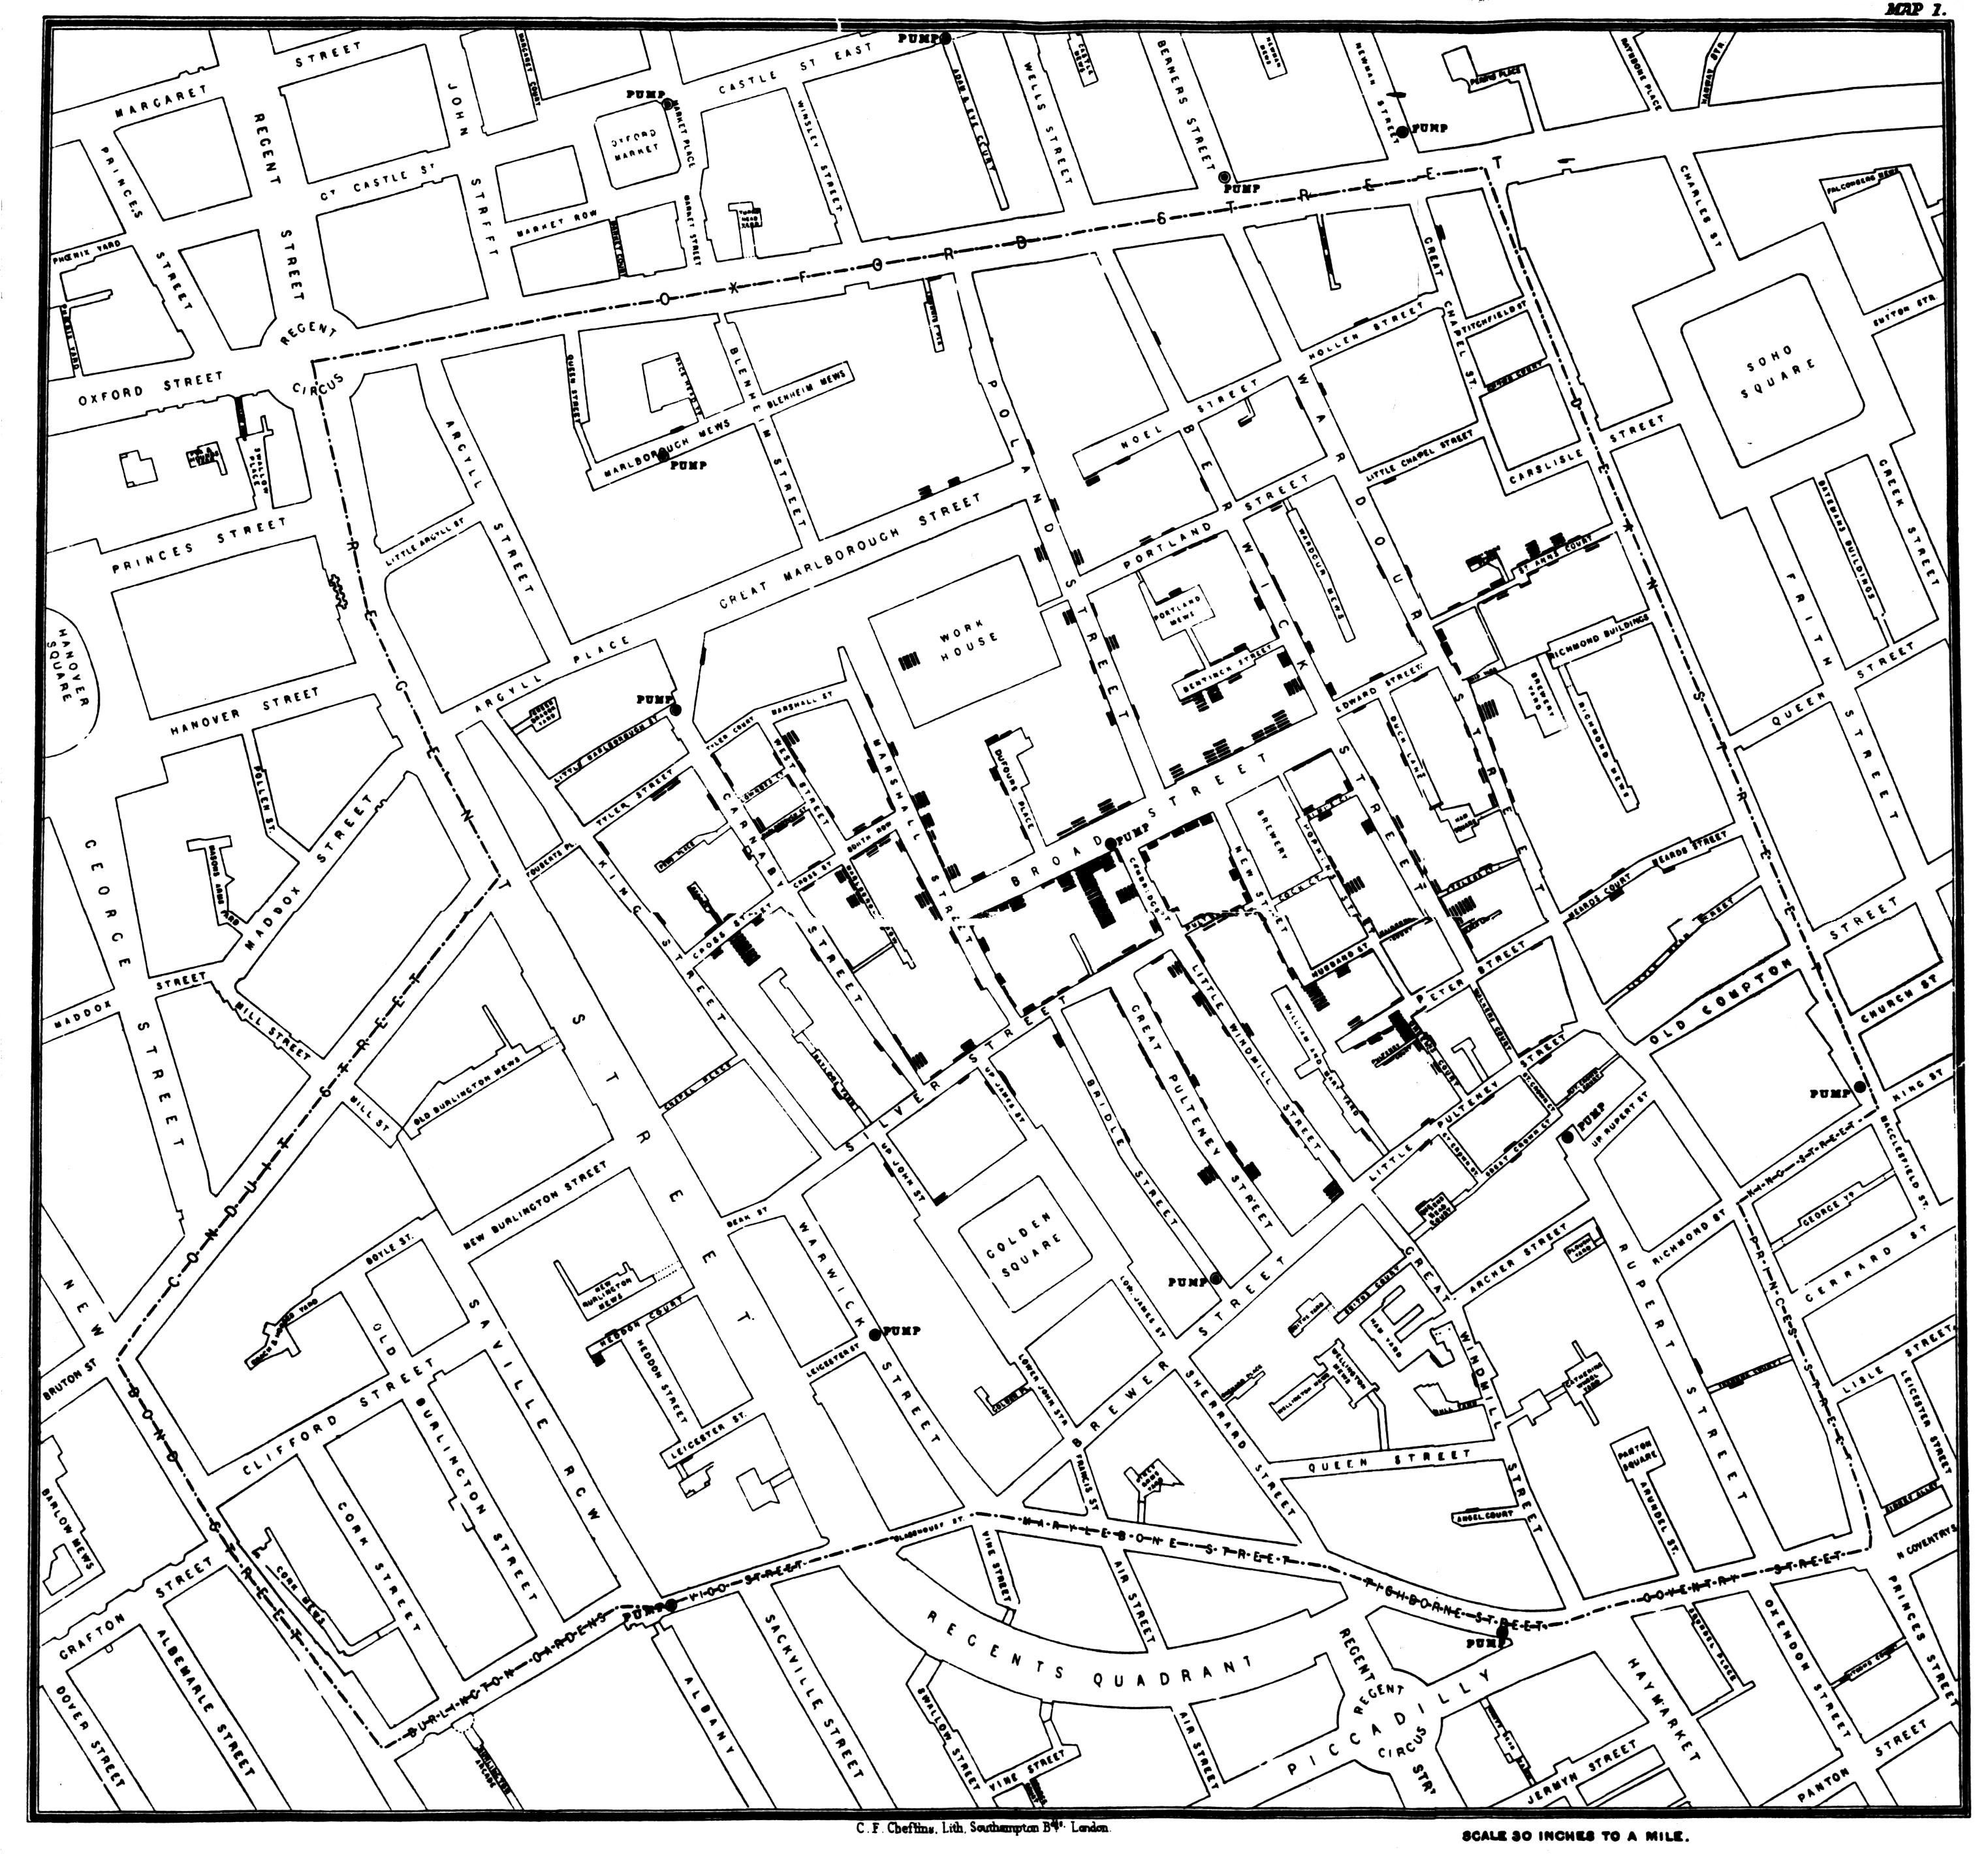
\includegraphics[scale=0.183]{Snow-cholera-map-1}
\caption{John Snow's original cholera map found in his publication ``On the Mode of Communication of Cholera" \cite{original}. Snow's map shows the spread of cholera in 1854, during the cholera outbreak. }
\label{fig:snow}
\end{figure}

Since Snow was particularly interested in whether cholera was a waterborne disease, he decided to map water pumps that were of interest to him, drawing black circles representing the locations of each water pump on the map. For each water pump, he labelled ``PUMP" in capitalised bold text. In addition, Snow made his map large enough to encapsulate water pumps in other vicinities considering the possibility that his hypothesis could be wrong. By doing this, it enabled Snow to distinguish and investigate any outliers or abnormalities of the outbreak which could be visualised on Snow's map \cite{blog}. Snow plotted each case of cholera on the map, drawing thin black strokes which formed horizontal bars. Each bar represented a death caused by cholera in the neighbourhood \cite{tedtalk}. Stacked horizontal bars, represented multiple deaths at a particular address ``like a pile of little corpses" \cite{blog}.

Snow's map not only allowed him to test his hypothesis of cholera being spread by contaminated water, but it also enabled Snow to visualise the statistical information he had collected in a meaningful way. If his hypothesis were true, then it was expected deaths from the cholera outbreak would cluster around a particular water source. 

\begin{figure}
\centering
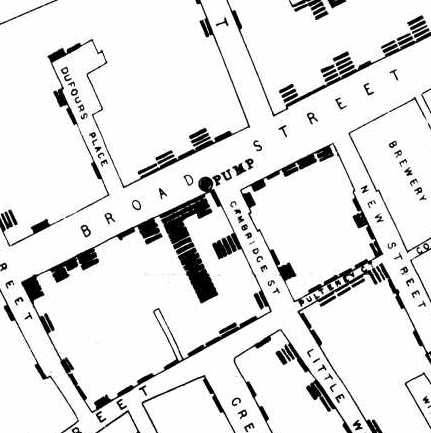
\includegraphics[scale=0.8]{snow_map_detail}
\caption{Snow's Cholera Map showing a detailed view of Broad Street where most cases of cholera occurred, each bar representing a fatality. }
\label{fig:snow}
\end{figure}

Since no one had listened to Snow, Snow created the map to attempt to convince doctors, scientists, authorities, and the general public that cholera was a waterborne disease. Since Snow's map was simple, it was relatively easy to understand given the meaning of the symbols, which are the black circles and horizontal bars (Shown in Figure 1 and Figure 2). Novice viewers such as the general public and local authorities could easily understand the visualisation, since Snow was able to convince authorities to remove the handle from the Broad Street pump. Expert viewers such as scientists and doctors also understood the map, and could see how the disease spread. 

Through the visualisation of the map, the message was evident. There was a significant amount of deaths clustered around a water pump on Broad Street (See Figure 2). This visualised ``something poisonous emanating out of this pump on the map" \cite{blog}, deaths further away from the map seemed to be getting less frequent (See Figure 1). The significance of Snow's map had changed the way we visualise disease such that ``many have said, changed medicine forever" \cite{heros}.

\section{The Significance of John Snow's Cholera Map}

John Snow was not the first to map the 1854 cholera outbreak \cite{history, johnson}. In 1832, Thomas Shapter used a dot map showing deaths caused by cholera in Europe \cite{howe1970some}. Despite this, Snow's map differed because it conveyed statistical information revealing patterns that could be linked back to the cause of the disease, testing Snow's hypothesis. In particular, it ``was the underlying science that the map revealed" \cite{johnson, history} which made it special.

John Snow used a scientific approach illustrating how it is possible to solve problems by visualising empirical evidence in a understandable way \cite{tedtalk}. Snow was able to link evidence from the cholera outbreak, and make logical connections providing a holistic view which explained what was happening \cite{channel1,blog}. Because of this, John Snow's technique of mapping the spread of disease is still used today \cite{channel1}. 

John Snow's cholera map evidently answers questions as to how cholera can affect a population, how it was spread, and the source in which it came from. It is evident as to what area cholera was most prominent, and which areas were not affected by cholera. From looking at the clustered regions of cholera on the map, it enabled the source causing the spread of cholera to be identified, in this case, the water pump on Broad Street. Although Snow's map answered questions regarding what was spreading cholera, it could not identify how cholera occurred in the first place, nor could identify what cholera actually was. Instead, Snow's map provided clues, enabling further investigation to be conducted to figure out the root cause of what truly triggered the cholera outbreak.  

Thanks to Snow's map, researchers later discovered that cholera was a waterborne disease caused by Vibrio cholerae, and that it was sewage that had leaked into the water pump on Broad Street which caused the cholera epidemic in 1854 \cite{channel1}. It had also convinced people of the change that they needed. Snow's map demonstrated the need for proper sanitary conditions during the nineteenth century, contributing to the health sector as it convinced London to fix their sewage system, ending cholera outbreaks \cite{top5}. Not only did his map affect public health, but it also affected the way data was visualised. By displaying ``medical statistics within a geographic image, a pattern of illness distribution was made visible in a way that pointed to its cause" \cite{test}. Today, these visualisations are called Geographic Information Systems (GIS) \cite{test}. Snow's map is said to be the birth of modern epidemiology: the study of disease and effects of health in a population \cite{youtube}. It is evident that Snow's map has made contributions to many fields, his technique of disease mapping still being used today \cite{channel1}. 

\section{Modern Visualisations}

John Snow's cholera map was considered to be a spot map: a map showing the geographic location of people that were affected by a disease, in this case, cholera. It was known as an early example of modern epidemiology, and demonstrated a way to map the spread of disease in a population. Since then, there have been adaptions to John Snow's cholera map. In the 1960's, a revised version of John Snow's map occurred in a cartography book. An illustrator, by the name of Regmarad, used a dot map, replacing bars with dots to represent deaths from cholera, shown in Figure \ref{fig:reg}  \cite{ralph}. However, in 1997, Eward Tufte explains as a dot map, Snow's map assumes ``the population in the area is uniformly distributed" \cite{blog}. The map assumes houses with no deaths have people living in them, as opposed to the house being empty altogether \cite{blog}. Despite this, Tufte praises Snow's map \cite{blog}.  

Since John Snow's original map, there have been developments in visualising geographical information through the use of computers, known as the field of Geographic Information Systems (GIS) \cite{howe1970some}. These maps can be used to visualise the spread of disease and visualise important patterns in data. The systems reduce the tedious work needed to map geographical information, and are reliable and efficient at processing information such as plotting data points and visualising these data points \cite{howe1970some}. In a published paper called ``Visualization and analytics tools for infectious disease epidemiology: A systematic review" it states that  ``these systems can help pinpoint cases and exposures, identify spatial trends, identify disease clusters, correlate different sets of spatial data, and test statistical hypotheses" \cite{recent}. 

Already there have been many adaptions to Snow's map in the field of GIS. Figure \ref{fig:gis} shows a revised version of Snow's map as a dot map Geographic Information System. Figure \ref{fig:gis1} is a Geographic Information System that visualises areas closet to each water pump as Theissen polygons. This enables information from Snow's map to be conveyed in a distinct way, highlighting areas of interest \cite{udel2}. A similar adaption shown in Figure \ref{fig:gis2} is a Geographic Information System showing the shortest travel distance via streets to each water pump \cite{udel2}. A modern adaption of Snow's map is shown in Figure \ref{fig:heatmap} as a Geographic Information System. The visualisation uses Kernel Density Estimation (KDE), which is a heat map, used to display the epidemic data from the 1854 cholera outbreak \cite{heatmap}. These are a few examples of adaptions made to Snow's map using GIS. 

Today, there are many mapping techniques used for visualising the spread of disease, similar to Snow's cholera map. Common mapping techniques used to visual disease have been achieved through dot maps, choropleth maps, isopleth maps, and gradient maps \cite{recent}. Modern visualisations mapping disease in GIS, provide fine granularity and dynamic functions. Already, there have been examples of adaptions to Snow's map that have dynamic features, enabling users to zoom into specific regions and examine details on demand (See Figure \ref{fig:gis_advanced}) \cite{advanced}. Similarly, there have also been other dynamic visualisations that are able to map multiple diseases as shown in Figure \ref{fig:recent} \cite{recent}. Users can select and choose the types of diseases that they want to visualise, which then dynamically displays the location and frequency of where the diseases are occurring. In future, it is expected adaptions of Snow's map will evolve to contain more fine grained controls and more information based on the direct users interacting with the system. Perhaps, users will be able to filter out specific cases, or reveal more information regarding each case from Snow's original map. We can only speculate how Snow's map will evolve, only time will tell. 

\begin{figure}
\centering
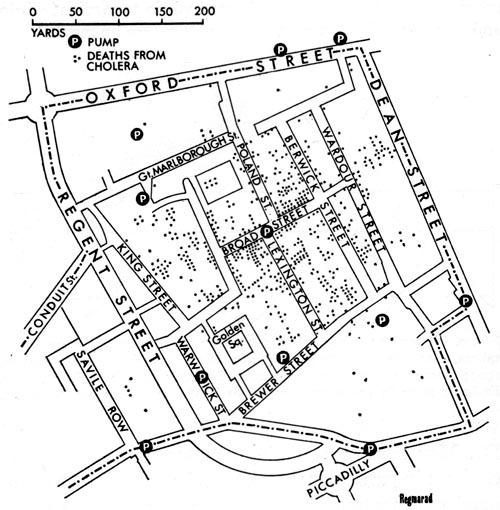
\includegraphics[scale=15.0]{snowmap1_regmarad}
\caption{Regmarad's version of a dot map based on Snow's cholera map \cite{ralph}.
}
\label{fig:reg}
\end{figure}

\begin{figure}
\centering
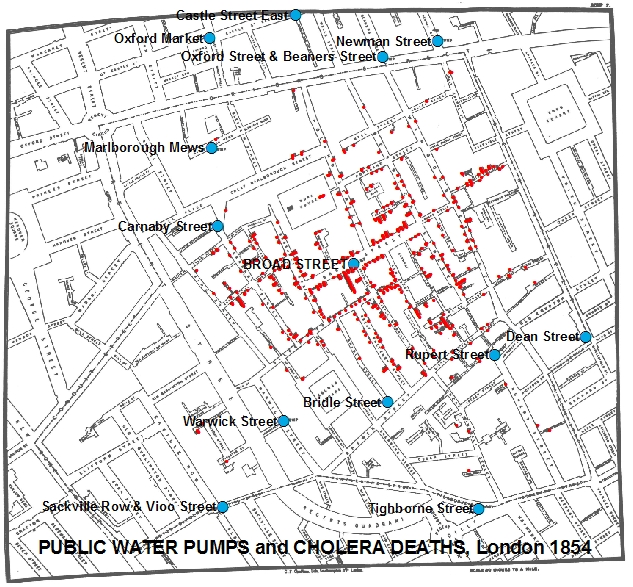
\includegraphics[scale=1.0]{gis}
\caption{A dot map generated by a Geographic Information System based on Snow's cholera map \cite{udel2}.}
\label{fig:gis}
\end{figure}

\begin{figure}
\centering
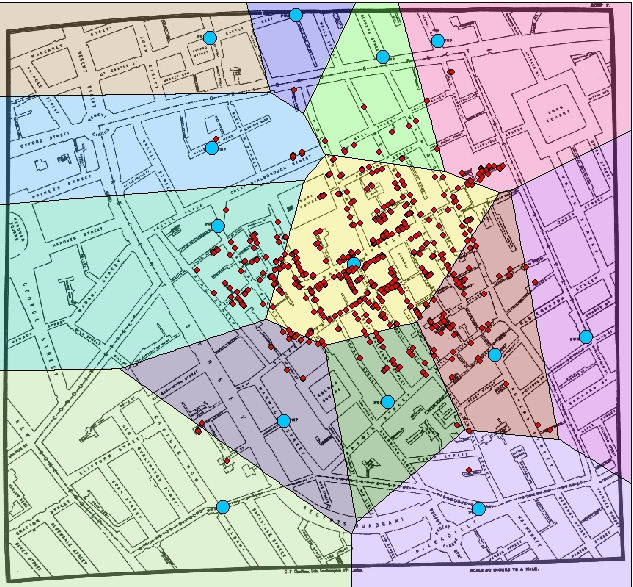
\includegraphics[scale=1.0]{gis_1}
\caption{ A Geographic Information System mapping areas (Theissen polygons) closest to each water pump based on Snow's cholera map \cite{udel2}.}
\label{fig:gis1}
\end{figure}

\begin{figure}
\centering
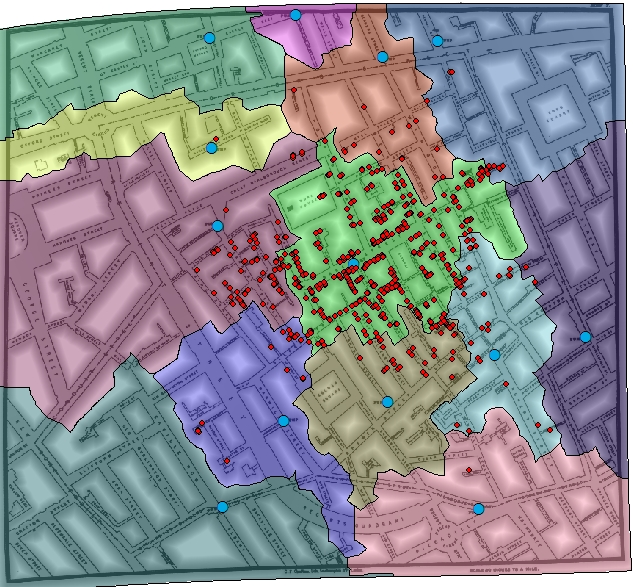
\includegraphics[scale=1.0]{gis_2}
\caption{
A Geographic Information System mapping areas based on the shortest distance (via streets) to each water pump based on Snow's cholera map \cite{udel2}.
}
\label{fig:gis2}
\end{figure}

\begin{figure}
\centering
\hspace*{-3cm}
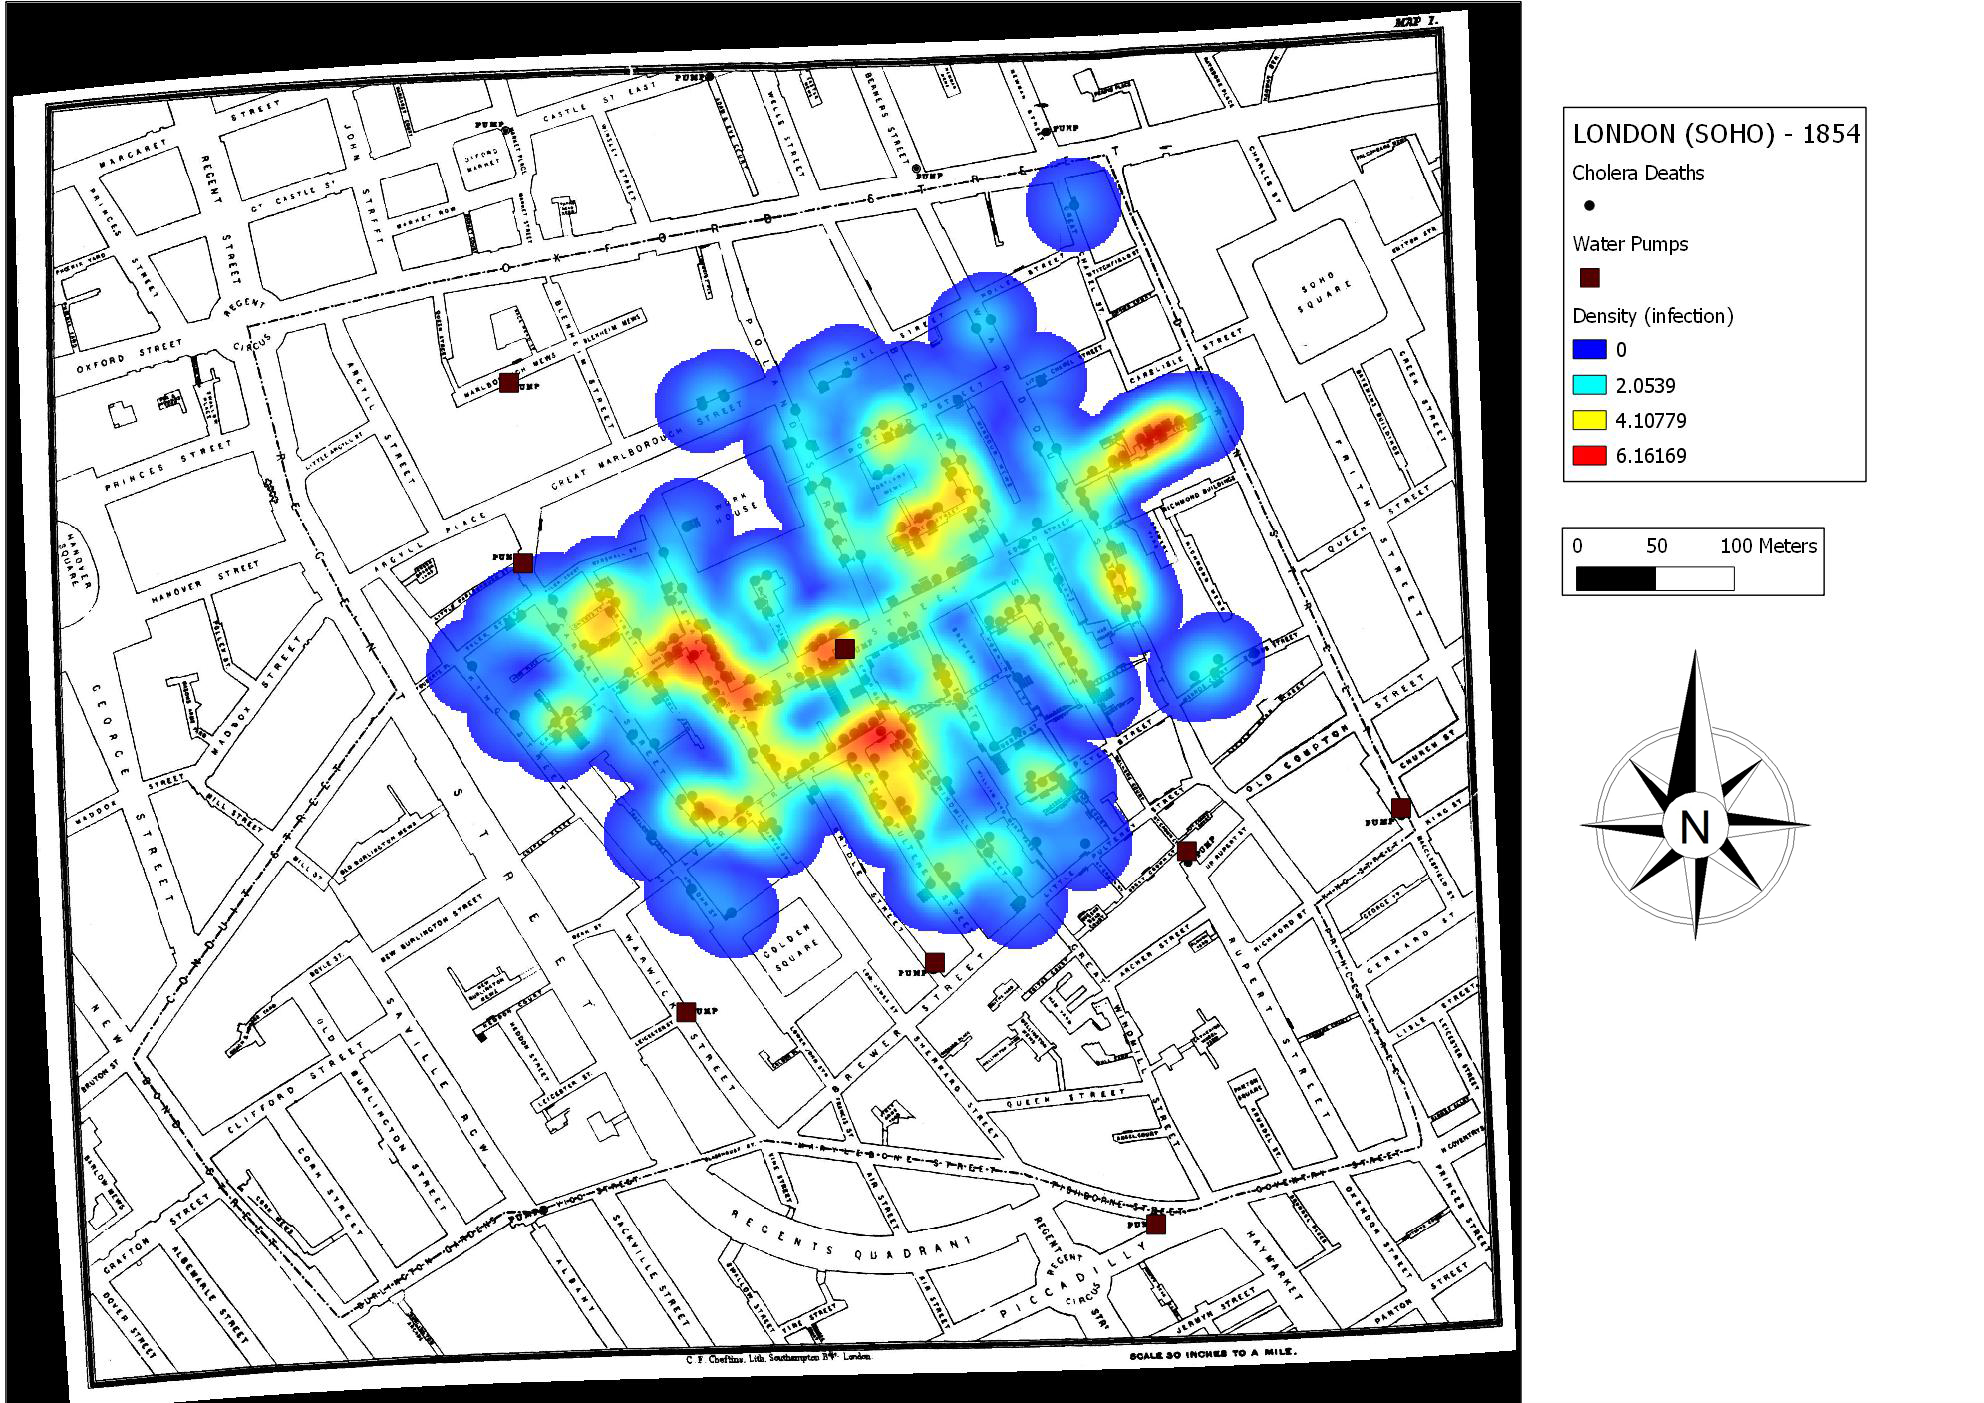
\includegraphics[scale=0.3]{gis_heatmap}
\caption{ 
A Geographic Information System displaying a heat map based on Snow's cholera map, the density proportional to deaths from cholera \cite{heatmap}.}
\label{fig:heatmap}
\end{figure}

\begin{figure}
\centering
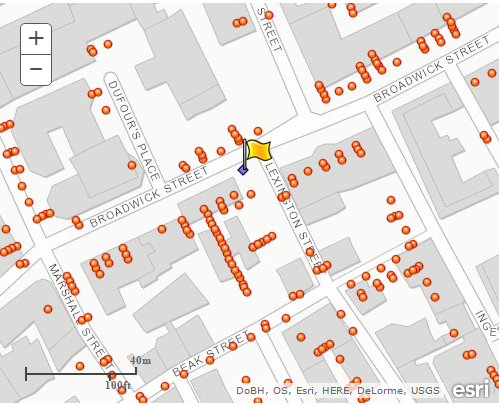
\includegraphics[scale=1.0]{gis_advanced}
\caption{A Geographic Information System based on Snow's cholera map. Users are able to zoom, pan, and hover over items to see details on demand \cite{advanced}.}
\label{fig:advanced}
\end{figure}


\begin{figure}
\centering
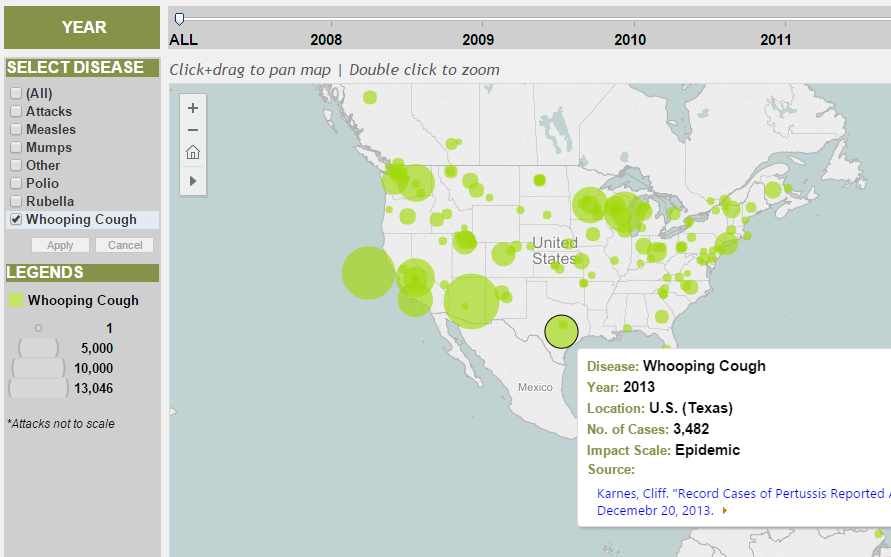
\includegraphics[scale=0.7]{recent}
\caption{A Geographic Information System that is able to map multiple diseases chosen by the user \cite{viz}. The user is able to filter diseases, choose a year, and hover over items to see details on demand.}
\label{fig:recent}
\end{figure}



\newpage

\bibliography{mybib}
\bibliographystyle{ieeetr}

\end{document}